\documentclass{beamer}
\usepackage{amsmath}
\usepackage{bm}
\usepackage{bbm}
\usepackage{amsfonts}
\usepackage{amssymb}
\usepackage{epsfig}

%\usepackage{beamerthemeJuanLesPins}  % quite good
%\usepackage{ beamerthemeMadrid}   % reasonable
%\usepackage{beamerthemeRochester} % very good, rectugularized
%\usepackage{beamerthemeSingapore} % very smooth and gives good space
%\usepackage{beamerthemeWarsaw} % excellent only the bottom problematic 
%\usepackage{}

%%%%%%%%%%%%%%%%%%%%%%%%%%%%%%%%%%%%%%%%%%%%%%%%%%%%%%%%%%%%%%%%%%%%
%
%  Utilities for typesetting in latex
%
%  Chris Williams, 1997, modified from utils.tex belonging to
%  Chris Bishop, 4 June 1995.
%
%
%%%%%%%%%%%%%%%%%%%%%%%%%%%%%%%%%%%%%%%%%%%%%%%%%%%%%%%%%%%%%%%%%%%%

\newcommand{\be}{\begin{equation}}
\newcommand{\ee}{\end{equation}}
\newcommand{\bi}{\begin{itemize}}
\newcommand{\ei}{\end{itemize}}
\newcommand{\bea}{\begin{eqnarray}}
\newcommand{\eea}{\end{eqnarray}}
\newcommand{\HOME}{/user/cs_neural/willicki}
%\newcommand{\COREL}{/user/cs_neural/bishopc/corel}

\newcommand{\bfdelta}{\boldsymbol{\delta}}
\newcommand{\bfDelta}{\boldsymbol{\Delta}}
\newcommand{\bfbeta}{\boldsymbol{\beta}}
\newcommand{\bfgamma}{\boldsymbol{\gamma}}
\newcommand{\bfmu}{\bm{\mu}}
%\newcommand{\bfmu}{\boldsymbol{\mu}}
\newcommand{\bfnu}{\boldsymbol{\nu}}
\newcommand{\bfalpha}{\boldsymbol{\alpha}}
\newcommand{\bfepsilon}{\boldsymbol{\epsilon}}
\newcommand{\bfSigma}{\boldsymbol{\Sigma}}
\newcommand{\bftau}{\boldsymbol{\tau}}
\newcommand{\bflambda}{\boldsymbol{\lambda}}
\newcommand{\bfLambda}{\boldsymbol{\Lambda}}
\newcommand{\bfpsi}{\boldsymbol{\psi}}
\newcommand{\bfxi}{\boldsymbol{\xi}}
\newcommand{\bfpi}{\bm{\pi}}
%\newcommand{\bfpi}{\boldsymbol{\pi}}
\newcommand{\bfPsi}{\boldsymbol{\Psi}}
\newcommand{\bfphi}{\boldsymbol{\phi}}
\newcommand{\bfPhi}{\boldsymbol{\Phi}}
\newcommand{\bfrho}{\boldsymbol{\rho}}
\newcommand{\bftheta}{\boldsymbol{\theta}}
\newcommand{\bfTheta}{\boldsymbol{\Theta}}
\newcommand{\bfomega}{\boldsymbol{\omega}}

\newcommand{\Bmath}[1]{\boldsymbol{#1}}

\newcommand{\bfa}{\mathbf{a}}
\newcommand{\bfb}{\mathbf{b}}
\newcommand{\bfc}{\mathbf{c}}
\newcommand{\bfd}{\mathbf{d}}
\newcommand{\bfe}{\mathbf{e}}
\newcommand{\bff}{\mathbf{f}}
\newcommand{\bfg}{\mathbf{g}}
\newcommand{\bfh}{\mathbf{h}}
\newcommand{\bfk}{\mathbf{k}}
\newcommand{\bfl}{\mathbf{l}}
\newcommand{\bfm}{\mathbf{m}}
\newcommand{\bfn}{\mathbf{n}}
\newcommand{\bfo}{\mathbf{o}}
\newcommand{\bfp}{\mathbf{p}}
\newcommand{\bfq}{\mathbf{q}}
\newcommand{\bfr}{\mathbf{r}}
\newcommand{\bfs}{\mathbf{s}}
\newcommand{\bft}{\mathbf{t}}
\newcommand{\bfu}{\mathbf{u}}
\newcommand{\bfv}{\mathbf{v}}
\newcommand{\bfw}{\mathbf{w}}
\newcommand{\bfx}{\mathbf{x}}
\newcommand{\bfy}{\mathbf{y}}
\newcommand{\bfz}{\mathbf{z}}

\newcommand{\bfzero}{\mathbf{0}}
\newcommand{\bfone}{\mathbf{1}}

\newcommand{\bfA}{\mathbf{A}}
\newcommand{\bfB}{\mathbf{B}}
\newcommand{\bfC}{\mathbf{C}}
\newcommand{\bfD}{\mathbf{D}}
\newcommand{\bfE}{\mathbf{E}}
\newcommand{\bfG}{\mathbf{G}}
\newcommand{\bfH}{\mathbf{H}}
\newcommand{\bfI}{\mathbf{I}}
\newcommand{\bfK}{\mathbf{K}}
\newcommand{\bfL}{\mathbf{L}}
\newcommand{\bfM}{\mathbf{M}}
\newcommand{\bfO}{\mathbf{O}}
\newcommand{\bfP}{\mathbf{P}}
\newcommand{\bfQ}{\mathbf{Q}}
\newcommand{\bfR}{\mathbf{R}}
\newcommand{\bfS}{\mathbf{S}}
\newcommand{\bfT}{\mathbf{T}}
\newcommand{\bfU}{\mathbf{U}}
\newcommand{\bfV}{\mathbf{V}}
\newcommand{\bfW}{\mathbf{W}}
\newcommand{\bfX}{\mathbf{X}}
\newcommand{\bfY}{\mathbf{Y}}
\newcommand{\bfZ}{\mathbf{Z}}
\newcommand{\llangle}{{\langle \vspace{-2mm} \langle}}
\newcommand{\rrangle}{{\rangle \vspace{-2mm} \rangle}}
\newcommand{\la}{\leftarrow}

\newcommand{\tf}{\tilde{f}}
\newcommand{\tg}{\tilde{g}}
\newcommand{\tX}{\tilde{X}}
\newcommand{\tY}{\tilde{Y}}
\newcommand{\tZ}{\tilde{Z}}

\newcommand{\bbE}{\mathbb{E}}
\newcommand{\bbR}{\mathbb{R}}
\newcommand{\bbP}{\mathbb{P}}
\newcommand{\bbT}{\mathbb{T}}
\newcommand{\bbZ}{\mathbb{Z}}

% for Fourier analysis
\newcommand{\ois}{2 \pi i s}  % ois is mnemonic for omega i of s
\newcommand{\oik}{2 \pi i k}  % ois is mnemonic for omega i of k
\newcommand{\oin}{2 \pi i n}  % ois is mnemonic for omega i of n
\newcommand{\oim}{2 \pi i m}  % ois is mnemonic for omega i of m

%\newcommand{\T}{\mathop{\rm T}\nolimits}
\newcommand{\T}{{\rm T}}
%\newcommand{\iint}{\int \! \! \int}
%\newcommand{\iiint}{\int \! \! \int \! \! \int}
\newcommand{\Tr}{\mbox{Tr}}
\newcommand{\diff}[1]{{\,d#1}}
\newcommand{\vgraph}[1]{
  \newpage
  \begin{center}
  {\large \bf #1}
  \end{center}
  \vspace{2mm}
}
%%\newcommand{\lapproxeq}{\stackrel{\textstyle <}{\sim}}
\newcommand{\high}[1]{\textcolor{blue}{\emph{#1}}}
\newcommand{\cut}[1]{}
\newcommand{\citeasnoun}[1]{\citeN{#1}}
\newcommand{\citemulti}[2]{(#1, \citeyearNP{#2})}
\newcommand{\citemultiN}[2]{#1 (\citeyearNP{#2})}
\newcommand{\Sum}{{\displaystyle \sum}}
\newcommand{\defeq}{{\stackrel{def}{=}}}
\newcommand{\marg}[1]{\marginpar{#1}}

%%%%%%%%%%%%%%%%%%%%%%%%%%%%%%%%%%%%%%%%%%%%%%%%%%%%%%%%%%%%%%%%%%%%

\newcommand{\pdt}[2]{\frac{\partial^2 #1}{\partial {#2}^2 }}
\newcommand{\pdsd}[3]{\frac{\partial^2 #1}{\partial {#2} \partial {#3} }}
\newcommand{\pdo}[2]{\frac{\partial {#1}}{\partial {#2}}}
\newcommand{\pdol}[2]{\partial {#1}/ \partial {#2}}
\newcommand{\pdu}[1]{\frac{\partial }{\partial {#1}}}                          

%%% Local Variables: 
%%% mode: latex
%%% TeX-master: t
%%% End: 


\title{Bayesian Gaussian Process Latent Variable Model}

\author{{\bf Michalis K. Titsias and  Neil D. Lawrence}\\ 
School of Computer Science, \\
University of Manchester}
\date{}


\begin{document}

\frame{\titlepage}


%\section[Outline]{}
%\frame{\tableofcontents}



\frame
{
\frametitle{Motivation}





\begin{itemize}

\item Gaussian processes are used for supervized learning
 
\begin{itemize} 

\item Inputs are fixed/\textcolor{red}{deterministic} 
      %But what is we have missing or uncertain inputs 
      %
      %But what if 
      %inputs are \textcolor{blue}{random}?   
       
\end{itemize}

\item Gaussian process latent variable model (GP-LVM) is trained  
      by optimizing (not marginalizing out) the latent variables 



\end{itemize}

\textcolor{blue}{We address the questions:}

\begin{itemize}

\item How can we train Gaussian process models when inputs are \textcolor{red}{random}
  (e.g.\ we have uncertain inputs/missing values)? 

\item How can we marginalize out the latent variables in GP-LVM?
      

%\begin{itemize}

%\item How can we apply a more full \textcolor{blue}{Bayesian} for
%  traning the GP-LVM where
%      latent variables are approximately \textcolor{blue}{marginalized out}? 

\end{itemize}



{\bf We will introduce a \textcolor{red}{variational Bayes} framework
 that provides approximate Bayesian solutions} 

%\begin{itemize}
%      
%      \item Deal with uncertain/missing inputs in GPs
%
%      \item Automatically select the dimensionality of the non-linear 
%            latent space in GP-LVM
% 
%      \item Learn non-parametric/non-linear 
%            dynamical systems (future work)    
% 
%\end{itemize} 

%\end{itemize} 

}




\frame
{
\frametitle{Outline}

\begin{itemize}

\item \textcolor{blue}{Variational inference} for GPs with random (uncertain/missing/latent) inputs 

\begin{itemize}

     \item The role of \textcolor{red}{auxiliary parameters} 

     \item The variational lower bound 
  
    % \item The 

    % \item Prediction 

\end{itemize} 

\item Variational inference for GP-LVM  

\begin{itemize}

  \item \textcolor{blue}{Automatic selection} of the latent
        dimensionality with the squared exponential ARD kernel 

\end{itemize} 

\item Experiments with GP-LVM

\item Summary 
 
\end{itemize} 

}


\frame
{

\frametitle{Gaussian Processes: Deterministic inputs}

\begin{itemize}

\item Gaussian process (GP) is used as non-parametric prior 
      over some function \textcolor{red}{$f(\bfx)$}
      %specified 
      %by mean and covaraince/kernel function 
      %$\small \mu(\bfx) = \mathbb{E}f(\bfx)$ and $k(\bfx,\bfx') =
      %\mathbbm{E}(f(\bfx)-\mu(\bfx))(f(\bfx') -\mu(\bfx'))$


%\item \textcolor{blue}{Supervised learning}: Estimate
%      regression functions, decision boundaries, intensities etc


\end{itemize}


\begin{columns}
\begin{column}[t]{8cm}

\begin{itemize}

\item \textcolor{blue}{Probability model:} Output-input data $(\bfy,X)$: 


\begin{eqnarray}
p(\bfy,\bff|X) & = &  p(\bfy|\bff) \times p(\bff|X) \nonumber \\
\text{\textcolor{red}{Joint}} & = & \text{\textcolor{red}{Likelihood}}
\times \text{\textcolor{red}{marginal GP on X}} \nonumber
\end{eqnarray}
where $X$ is assumed deterministic 
% Posterior process %$p(f(\cdot)|\bfy)$
%is Gaussian when $p(\bfy|\bff)$ is Gaussian
 
\end{itemize}

\end{column}

\begin{column}[t]{2cm}
\begin{figure}
%\begin{l}
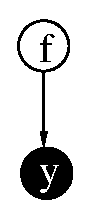
\includegraphics[width=7mm,height=20mm]{../../../vargplvm/tex/diagrams/net1}
%\end{l}
\end{figure}

\end{column}
\end{columns}

\vspace{0.3cm}

%\textcolor{red}
{\bf But what if the inputs $X$ are random?}

}



\frame
{

\frametitle{Gaussian Processes: Random inputs}



\begin{columns}
\begin{column}[t]{8cm}

\begin{itemize}
\item \textcolor{blue}{Probability model:} As before, but now the inputs $X$ 
        are given a prior (e.g.\ Gaussian) distribution  \textcolor{red}{$p(X)$}: 

$$
p(\bfy,\bff,X) =  p(\bfy|\bff) p(\bff|X) \textcolor{red}{p(X)} 
$$


\end{itemize}

\end{column}

\begin{column}[t]{2cm}
\begin{figure}
%\begin{l}
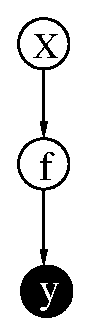
\includegraphics[width=8mm,height=33mm]{../../../vargplvm/tex/diagrams/net}
%\end{l}
\end{figure}

\end{column}
\end{columns}

%\vspace{0.3cm}

\begin{itemize}

%\item \textcolor{blue}{Random inputs} can be: 
%
%
%\begin{itemize}
%
%\item \textcolor{blue}{Uncertain inputs}, i.e.\ noisy input measurements
%
%\item \textcolor{blue}{Missing values} in $X$
%
%\item \textcolor{blue}{Latent variables} in non-linear probabilistic PCA 
%      (GP-LVM) 
%
%\end{itemize}

\item The \textcolor{red}{posterior} distribution $p(\bff,X|\bfy)$ and the \textcolor{red}{marginal 
      likelihood} $p(\bfy)$ are \textcolor{red}{intractable} 

\item \textcolor{blue}{Approximate inference:} Can we apply 
some standard variational  method? 
 

\end{itemize}


%\textcolor{red}
%{\bf Can we apply the standard mean field approximation?}


}



\frame
{

\frametitle{Variational inference: Difficult to apply}


\begin{itemize}

\item Standard regression with random inputs:

$$
p(\bfy,\bff,X) = \mathcal{N}(\bfy|\bff,\sigma^2 I) 
\textcolor{red}{p(\bff|X)} p(X) 
$$

$$
p(\bfy,\bff,X) = \mathcal{N}(\bfy|\bff,\sigma^2
  I) \textcolor{red}{\frac{1}{(2\pi)^{n/2} |K_{NN}|^{1/2}} 
e^{-\frac{1}{2} \bff^T K_{NN}^{-1}\bff}} p(X) 
$$

%where $p(\bff|X) = \mathcal{N}(\bff|\bfzero, K_{NN})$ and $p(X)$ 
%Gaussian


\item Applying mean field $q(\bff,X) = q(\bff) q(X)$
      is difficult:

      \begin{itemize}

       \item \textcolor{blue}{$X$ appears non-linearly inside the  inverse
             $K_{NN}^{-1}$ and the determinant $|K_{NN}|$} 
       
       \item Seems impossible to compute the variational bound 
               $\int q(\bff,X) \log \frac{p(\bfy,\bff,X)}{ q(\bff,X)}
               d \bff d X$ 
 

      \end{itemize}       

%\item Let's try to understand this 
%using the simplest possible example: 
%\textcolor{blue}{Bayesian linear regression} 

%      \begin{itemize}
%
%       \item Augment with a finite set of auxiliary parameters 
%
%\begin{itemize}
%
%       \item These will be extra points of the function $f(\bfx)$
%         called inducing variables 
%           
%\end{itemize}
% 
%      \end{itemize}
%

\end{itemize}

%{\bf But why we need auxiliary parameters?}

}



\frame
{

\frametitle{Variational inference: Bayesian Linear Regression}

Intractability even for the simplest model: 
\textcolor{blue}{Bayesian linear regression}

\begin{itemize} 

\item Standard parameters: 

      $$
      \bfy = X \bfw + \bfepsilon, \ \ N(\bfw|\bfzero, \sigma_w^2
      I), p(X)
      $$
     
     \begin{itemize}
      \item It is straightforward to apply mean field 
            using $q(\bfw)q(X)$
     \end{itemize}
      
\item \textcolor{red}{Kernelized} (non-parametrized):

       
      $$
      \bfy = \bff + \bfepsilon, \ \  N(\bff|\bfzero, \sigma_w^2
      XX^T), p(X)
      $$
     
      %where the  GP prior has a linear kernel  

\begin{itemize}

 \item Variational inference using $q(\bff) q(X)$ is difficult

\end{itemize}

%\item The kernelization makes  % on $X$ intractable 
%
%       \begin{itemize}
%            \item \textcolor{red}{$X$ appears in the inverse of $X X^T$} 
%               %cannot be integrated out (neither exactly nor
%               %variationally)
%
%             \item Not clear how to apply mean field using 
%                   $q(\bff) q(X)$
%
%       \end{itemize}
%
%
%  \item But if we keep $\bfw$, then
%    variational inference %in the space of $(\bfw,X)$
% is tractable  

\end{itemize}

}



\frame
{

\frametitle{Variational inference: Kernelization}


\begin{itemize} 


\item Gaussian processes (kernel methods in general) are somehow 
\textcolor{blue}{marginalized (collapsed)} 
      

\begin{itemize} 

\item A GP is an \textcolor{blue}{exchangeable} model:

 $$
 p(f_1,\ldots,f_N) = \int \prod_{n=1}^N p(f_n|\bfw) d P(\bfw)
 $$
 
 where the underlying (infinite) parameter $\bfw$ has been integrated out 

%\item We are left with the kernel function and \textcolor{blue}{inputs that 
%    appear inside matrix inverses} \textcolor{red}{$\Rightarrow$ intractability} 
  

\end{itemize}
 
\item We need to \textcolor{blue}{place back} some (approximate) parameters 
to apply  variational inference. We will use \textcolor{red}{extra function 
values} as parameters

%\item These parameter will be auxiliary function points 
%      called inducing variables 

\end{itemize}

%{\bf The parameters we use are auxiliary function points used in sparse
%  GPs, called inducing variables}

}




\frame
{

\frametitle{Variational inference: The idea} 

\begin{columns}
\begin{column}[t]{8cm}

\begin{itemize}
\item Initial model:
$$
p(\bfy,\bff,X) = \mathcal{N}(\bfy|\bff,\sigma^2
  I) p(\bff|X) p(X) 
$$
(\textcolor{blue}{variational inference in $(\bff,X)$ is difficult})

\end{itemize}
\end{column}

\begin{column}[t]{3cm}
\begin{figure}
%%\begin{l}
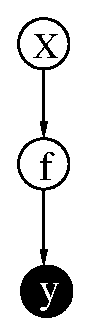
\includegraphics[width=8mm,height=30mm]{../../../vargplvm/tex/diagrams/net}
%\end{l}
\end{figure}
\end{column}
\end{columns}

\begin{columns}
\begin{column}[t]{8cm}
\begin{itemize}

\item Augment \textcolor{red}{consistently}\footnote{$\int
    p(\bff|\bfu, X) p(\bfu) d \bfu =
    p(\bff|X)$, for any value of inputs $Z$}
 with extra function values $\bfu = (f(\bfz_1),\ldots,f(\bfz_M))$:

\begin{eqnarray}
p(\bfy,\bff,\bfu, X) 
%& = & 
%\mathcal{N}(\bfy|\bff,\sigma^2I)
%\textcolor{red}{p(\bff,\bfu| X)} p(X) \nonumber \\
& = & \mathcal{N}(\bfy|\bff,\sigma^2I)
\textcolor{red}{p(\bff | \bfu, X) p(\bfu)} p(X) \nonumber
\end{eqnarray}

(\textcolor{blue}{variational inference in $(\bff, \bfu, X)$ is tractable})

\end{itemize}
\end{column}
\begin{column}[t]{3cm}
\begin{figure}
%%\begin{l}
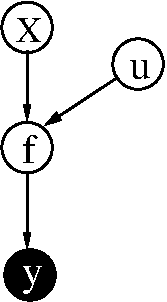
\includegraphics[width=20mm,height=30mm]{../../../vargplvm/tex/diagrams/net2}
%\end{l}
\end{figure}
\end{column}
\end{columns}

}



%\frame
%{
%
%\frametitle{Inducing variables: Linear GP} 
%
%
%%Inducing variables can replace the standard parameter $\bfw$ 
%%in PCA  and allow for variational inference in the kernelized model 
%
%\begin{figure}
%%\begin{l}
%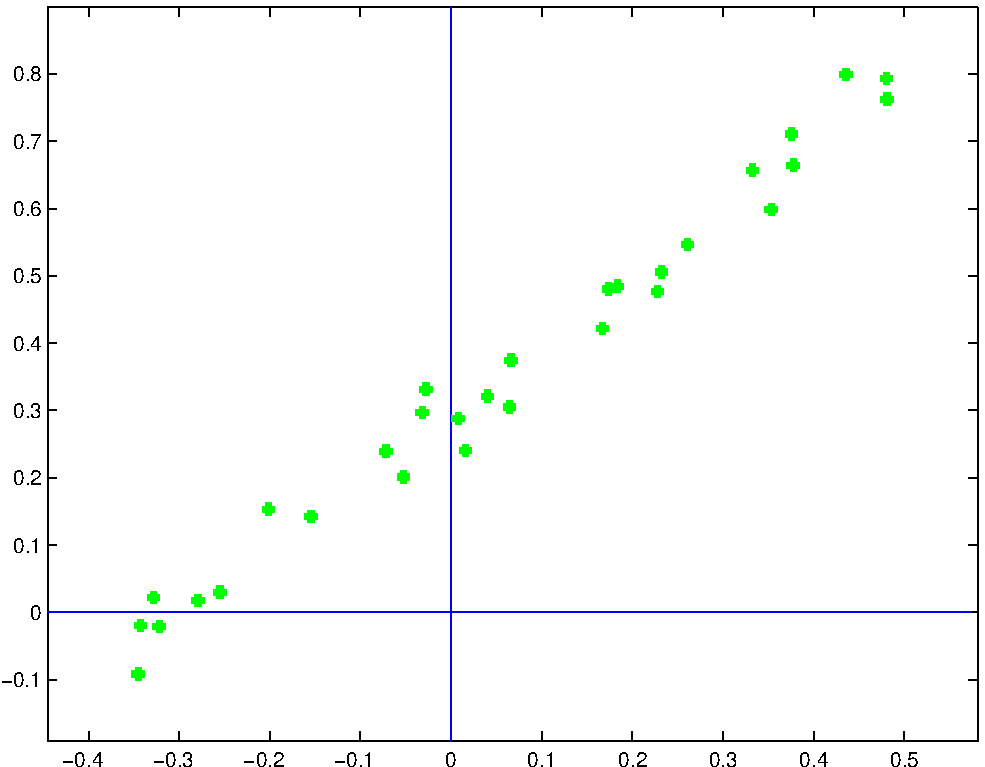
\includegraphics[width=55mm,height=50mm]{../../../vargplvm/tex/diagrams/Fig11}
%%\end{l}
%\end{figure}
%
%\begin{itemize}
%
%\item Illustration of augmented GP with inducing variables:
%
%$$ 
%p(\bfy,\bff,\bfu, X) = \mathcal{N}(\bfy|\bff,\sigma^2I)
%p(\bff | \bfu, X) p(\bfu) p(X)
%$$
%
%\end{itemize}
%
%
%} 


%\frame
%{
%
%\frametitle{Inducing variables: Linear GP} 
%
%%Inducing variables can replace the standard parameter $\bfw$ 
%%in PCA  and allow for variational inference in the kernelized model 
%
%Visualization of the augmented GP model and the inducing variables
%
%\begin{figure}
%%\begin{l}
%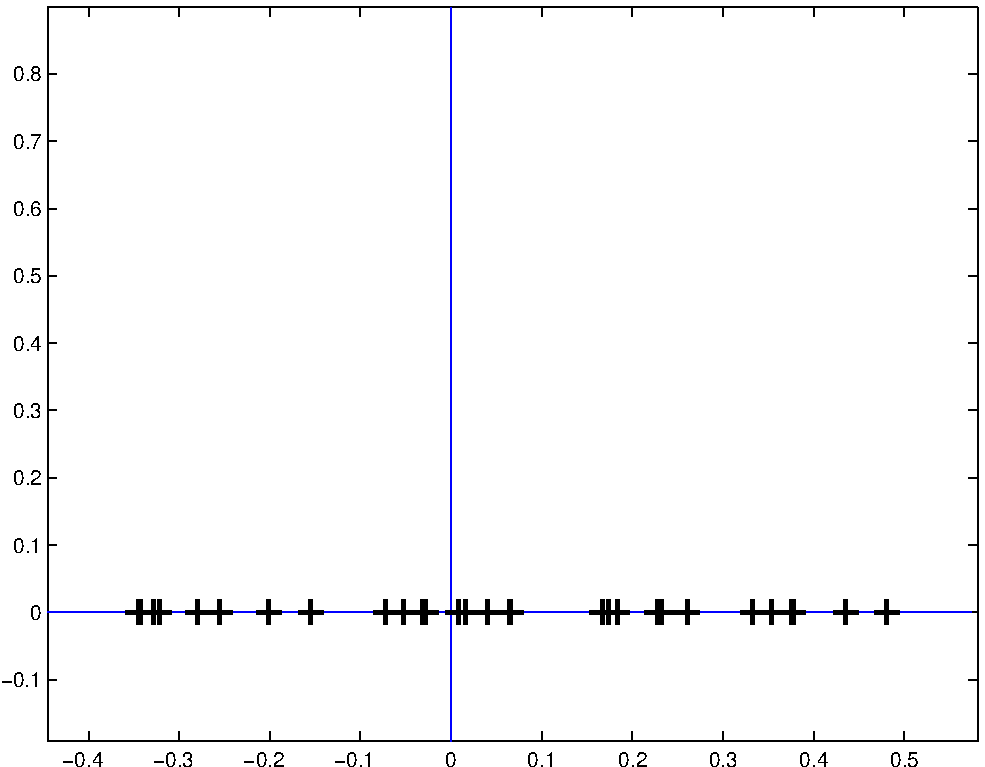
\includegraphics[width=55mm,height=50mm]{../../../vargplvm/tex/diagrams/Fig2}
%%\end{l}
%\end{figure}
%
%
%\begin{itemize}
%
%\item Draw input data $X$:
%
%$$ 
%p(\bfy,\bff,\bfu, X) = \mathcal{N}(\bfy|\bff,\sigma^2I)
%p(\bff | \bfu, X) p(\bfu) \textcolor{blue}{p(X)}
%$$
%
%\end{itemize}
%
%
%} 
%
%
%\frame
%{
%
%\frametitle{Inducing variables: Linear GP} 
%
%%Inducing variables can replace the standard parameter $\bfw$ 
%%in PCA  and allow for variational inference in the kernelized model 
%
%\begin{figure}
%%\begin{l}
%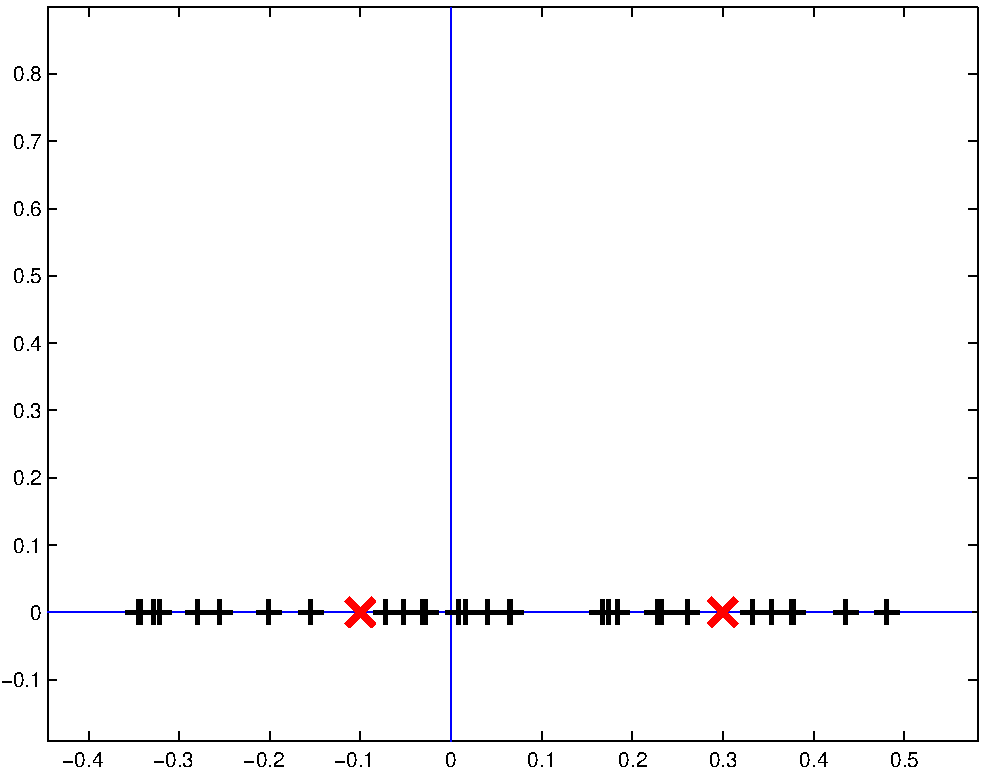
\includegraphics[width=55mm,height=50mm]{../../../vargplvm/tex/diagrams/Fig3}
%%\end{l}
%\end{figure}
%
%\begin{itemize}
%
%\item Choose some pseudo (unrelated to $X$) inputs $Z$ 
%
%$$ 
%p(\bfy,\bff,\bfu, X) = \mathcal{N}(\bfy|\bff,\sigma^2I)
%p(\bff | \bfu, X) p(\bfu) p(X)
%$$
%
%\end{itemize}
%
%\textcolor{red}{\bf Crucial: $Z$ are not random variables}
%
%
%} 
%
%
%\frame
%{
%
%\frametitle{Inducing variables: Linear GP} 
%
%%Inducing variables can replace the standard parameter $\bfw$ 
%%in PCA  and allow for variational inference in the kernelized model 
%
%\begin{figure}
%%\begin{l}
%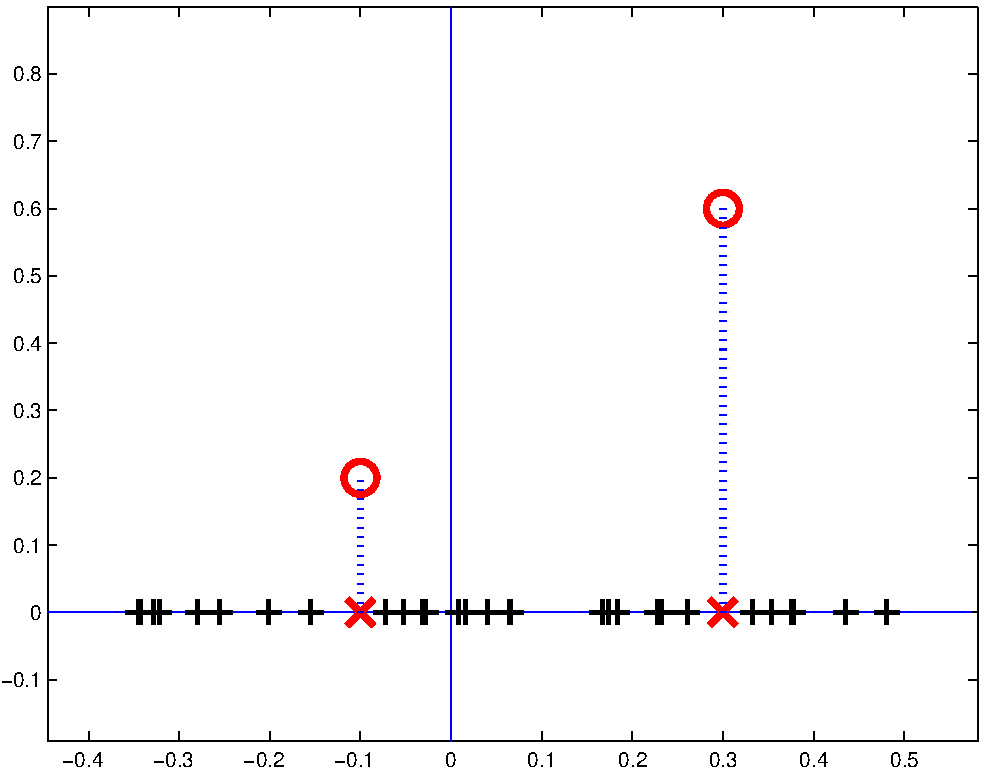
\includegraphics[width=55mm,height=50mm]{../../../vargplvm/tex/diagrams/Fig4}
%%\end{l}
%\end{figure}
%
%\begin{itemize}
%
%\item Sample random function values $\bfu$ at the pseudo-inputs $Z$ 
%
%$$ 
%p(\bfy,\bff,\bfu, X) = \mathcal{N}(\bfy|\bff,\sigma^2I)
%p(\bff | \bfu, X)  \textcolor{blue}{p(\bfu)} p(X)
%$$
%
%where $p(\bfu) = \mathcal{N}(\bfu|\bfzero, Z Z^T)$ 
%
%\end{itemize}
%
%}
%
%
%\frame
%{
%
%\frametitle{Inducing variables: Linear GP} 
%
%%Inducing variables can replace the standard parameter $\bfw$ 
%%in PCA  and allow for variational inference in the kernelized model 
%
%\begin{figure}
%%\begin{l}
%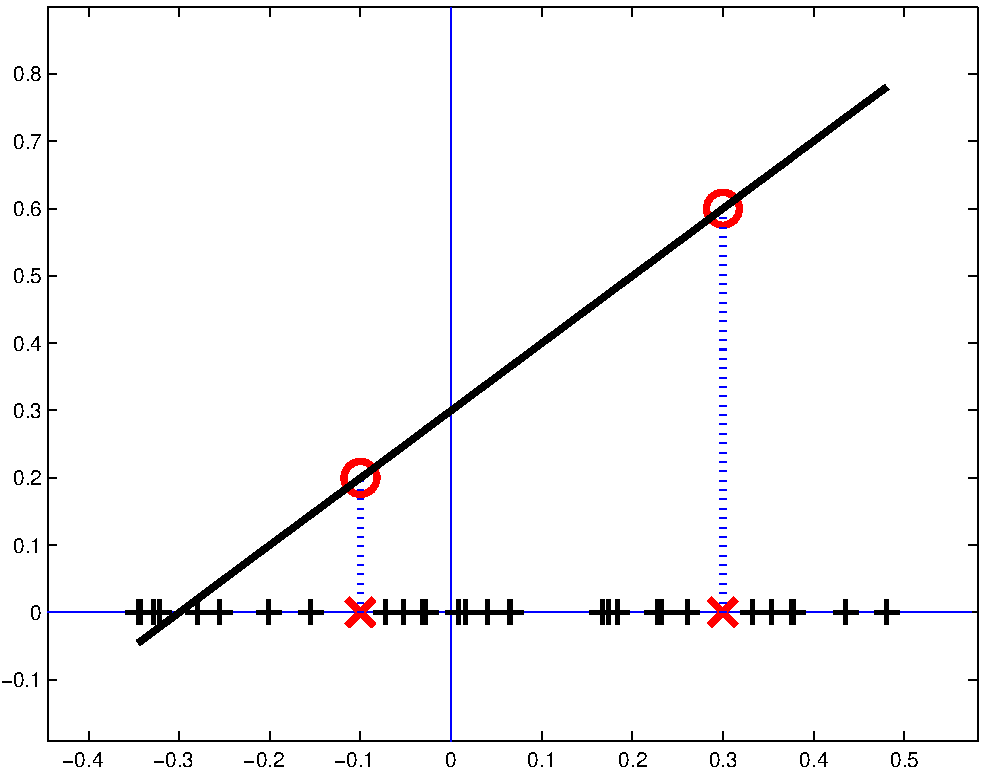
\includegraphics[width=55mm,height=50mm]{../../../vargplvm/tex/diagrams/Fig5}
%%\end{l}
%\end{figure}
%
%\begin{itemize}
%
%\item Sample function values $\bff$ on training inputs $X$
%      so that the function passes from the inducing variables 
%             
%$$ 
%p(\bfy,\bff,\bfu, X) = \mathcal{N}(\bfy|\bff,\sigma^2I)
% \textcolor{blue}{p(\bff | \bfu, X)} p(\bfu) p(X)
%$$
% 
%(\textcolor{red}{$p(\bff | \bfu, X)$ is the delta function in the example!})
%
%\end{itemize}
%
%}


\frame
{

\frametitle{Visualization} 

%Inducing variables can replace the standard parameter $\bfw$ 
%in PCA  and allow for variational inference in the kernelized model 

\begin{figure}
%\begin{l}
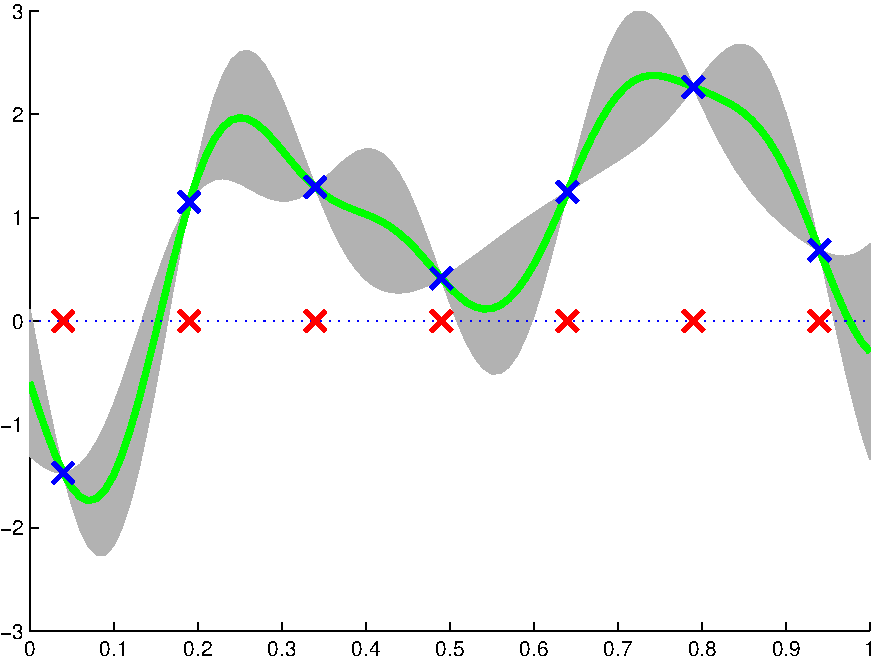
\includegraphics[width=55mm,height=45mm]{../../../vargplvm/tex/diagrams/Ind1}
%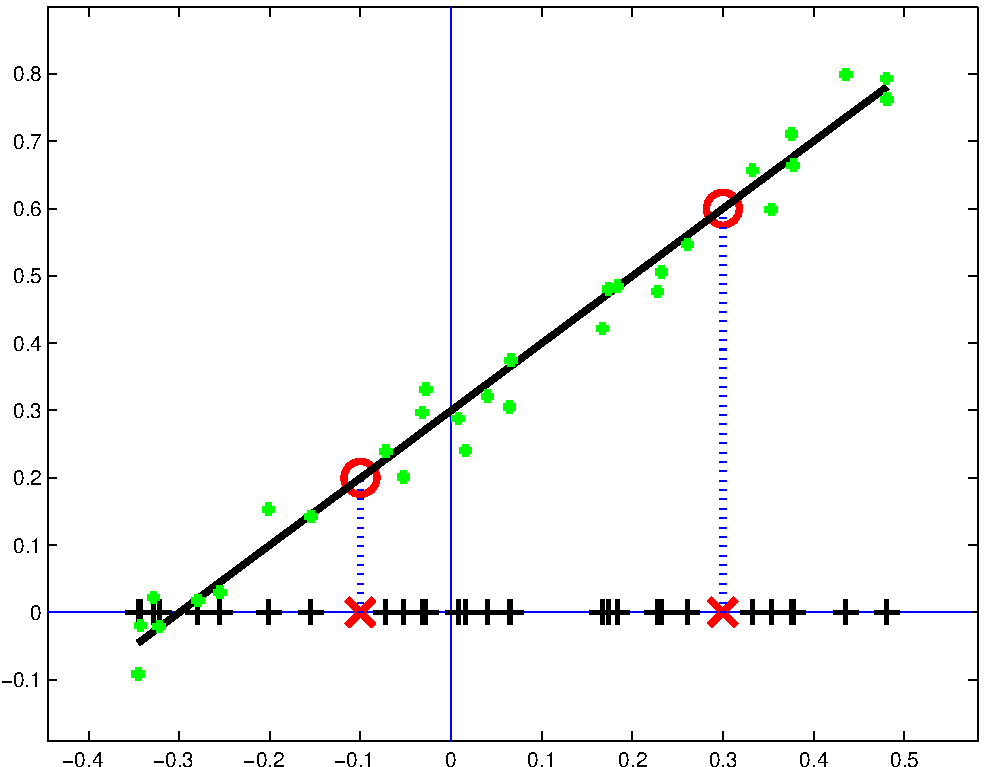
\includegraphics[width=55mm,height=50mm]{../../../vargplvm/tex/diagrams/Fig6}
%\end{l}
\end{figure}

\begin{itemize}

\item \textcolor{blue}{Blue Xs}: extra function points $\bfu$
\item \textcolor{red}{Red Xs}: inputs of  extra function points
\item \textcolor{green}{Green curve}: function $\bff$ drawn from 
      $p(\bff|\bfu,X)$
\item {\bf Shaded area:} conditional GP prior $p(\bff|\bfu,X)$


%\item Generate the observed data $\bfy$             
%
%$$ 
%p(\bfy,\bff,\bfu, X) = \textcolor{blue}{\mathcal{N}(\bfy|\bff,\sigma^2I)}
%   p(\bff | \bfu, X) p(\bfu) p(X)
%$$
% 

\end{itemize}


}


\frame
{

\frametitle{Visualization} 


\begin{figure}
%\begin{l}
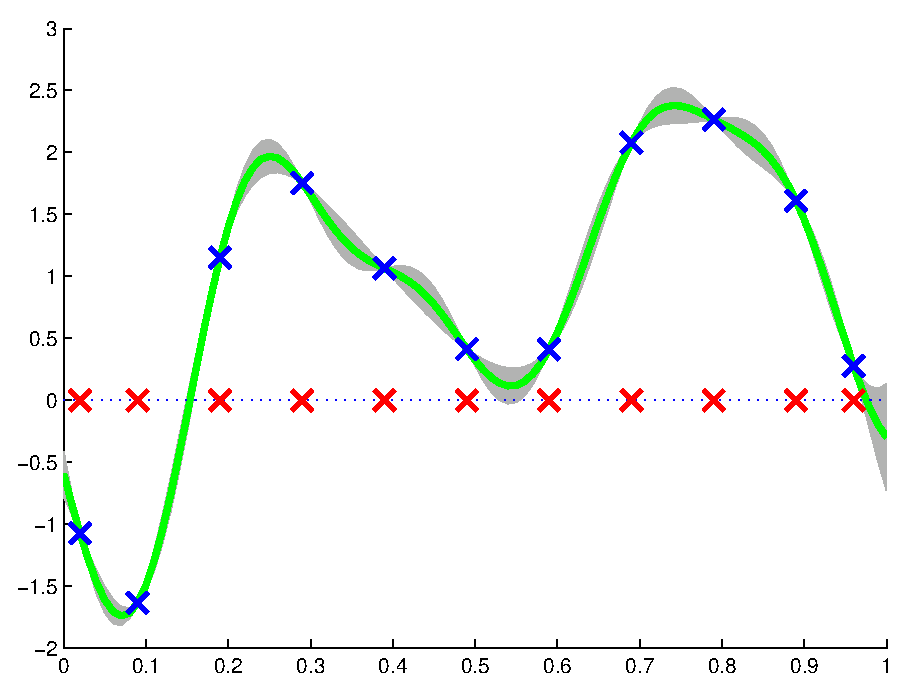
\includegraphics[width=55mm,height=45mm]{../../../vargplvm/tex/diagrams/Ind2}
%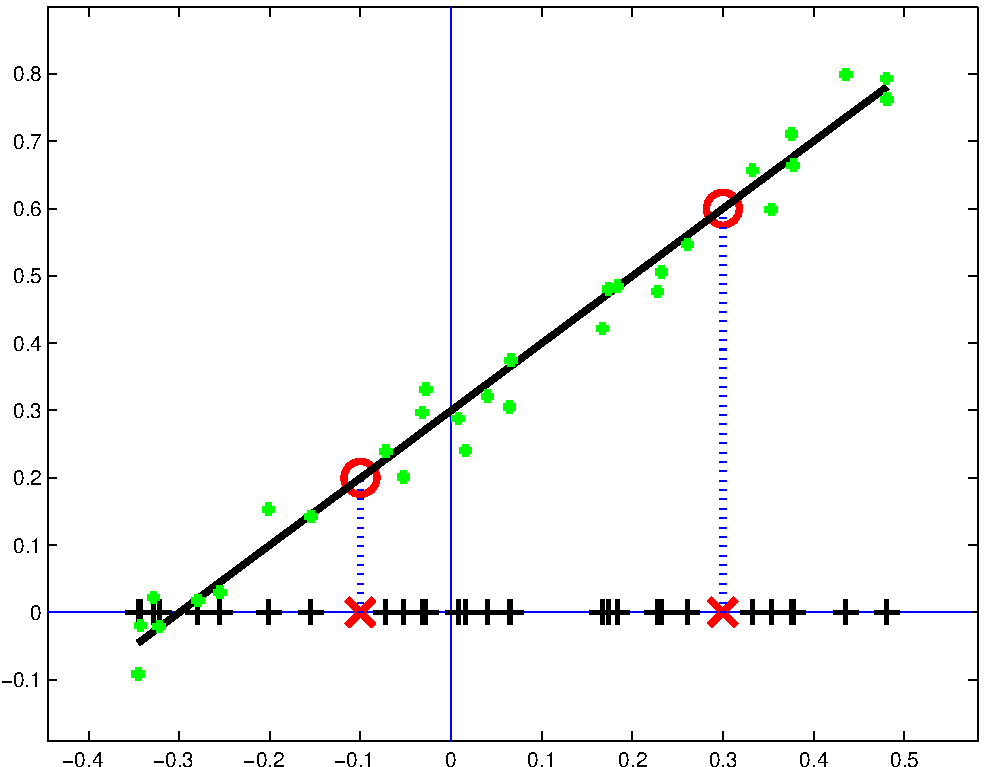
\includegraphics[width=55mm,height=50mm]{../../../vargplvm/tex/diagrams/Fig6}
%\end{l}
\end{figure}

\begin{itemize}

\item You can think of $\bfu$ as a parameter that 
      specifies the function $\bff$

\item When I use more  points in $\bfu$, 
      $p(\bff|\bfu,X)$ becomes more certain, i.e.\ 
      the parameter $\bfu$ is more informative

\item If the kernel is linear, $2$ points $(u_1,u_2)$
      fully specify an 1-D function (\textcolor{blue}{$p(\bff|\bfu,X)$ 
      becomes the delta function})
      


\end{itemize}

}


\frame
{

\frametitle{Variational inference} 

\begin{columns}
\begin{column}[t]{8cm}

\begin{itemize}
\item Initial model:
$$
p(\bfy,\bff,X) = \mathcal{N}(\bfy|\bff,\sigma^2
  I) p(\bff|X) p(X) 
$$

\end{itemize}
\end{column}

\begin{column}[t]{3cm}
\begin{figure}
%%\begin{l}
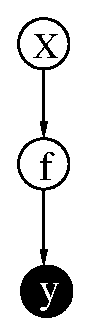
\includegraphics[width=8mm,height=30mm]{../../../vargplvm/tex/diagrams/net}
%\end{l}
\end{figure}
\end{column}
\end{columns}

\begin{columns}
\begin{column}[t]{8cm}
\begin{itemize}

\item Augmented model:

\begin{eqnarray}
p(\bfy,\bff,\bfu, X) 
%& = & 
%\mathcal{N}(\bfy|\bff,\sigma^2I)
%p(\bff,\bfu| X) p(X) \nonumber \\
& = & \mathcal{N}(\bfy|\bff,\sigma^2I)
\textcolor{red}{p(\bff | \bfu, X) p(\bfu)} p(X) \nonumber
\end{eqnarray}

\end{itemize}
\end{column}
\begin{column}[t]{3cm}
\begin{figure}
%%\begin{l}
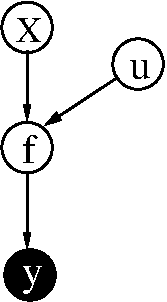
\includegraphics[width=20mm,height=30mm]{../../../vargplvm/tex/diagrams/net2}
%\end{l}
\end{figure}
\end{column}
\end{columns}

\vspace{0.2cm}
{\bf We apply variational inference in the space of $(\bff, \bfu, X)$}

}

\frame
{

\frametitle{Variational inference}


\begin{itemize}

%\item True posterior distribution: $
%p(\bff, \bfu, X) = p(\bff|\bfu, \bfy, X) p(\bfu,X|\bfy)
%$

\item Variational distribution: 

$$q(\bff, \bfu, X) = \textcolor{magenta}{p(\bff|\bfu, X)} \phi(\bfu) q(X)$$

\begin{itemize}


%\item It is mean field w.r.t.\  to $\bfu$ and $q(X)$

%\item The best   

\item $q(X)=\mathcal{N}(\bfmu,\Sigma)$: Gaussian distribution

\item $\phi(\bfu)$: unrestricted (turns out to be Gaussian) 

\item $p(\bff|\bfu, X)$: conditional  GP prior (\textcolor{magenta}{\bf trick})

%\item It is mean field  w.r.t.\ $\bfu$ and $X$

\end{itemize}


\item Maximize the lower bound

\begin{multline}
 \log \int \mathcal{N}(\bfy|\bff,\sigma^2 I) 
p(\bff|\bfu, X) p(X) d \bff d \bfu \bfX \geq \\
\int p(\bff|\bfu, X) \phi(\bfu) q(X)  
\log \frac{\mathcal{N}(\bfy|\bff,\sigma^2 I) 
\textcolor{red}{p(\bff|\bfu, X)} p(\bfu) p(X)}
{ \textcolor{red}{p(\bff|\bfu, X)} \phi(\bfu) q(X)} d \bff d \bfu \bfX
\nonumber 
\end{multline}
%or
%$$
%= \int p(\bff|\bfu, X) \phi(\bfu) q(X)  
%\log \frac{\mathcal{N}(\bfy|\bff,\sigma^2 I) p(\bfu) p(X)}
%{\phi(\bfu) q(X)} d \bff d \bfu \bfX
%$$

\end{itemize}

where \textcolor{red}{$p(\bff|\bfu, X)$s} inside the log cancel

\textcolor{blue}{\bf This is now tractable. Matrix inverses containing $X$ are gone}


}






\frame
{

\frametitle{Variational inference}

$$
\int p(\bff|\bfu, X) \phi(\bfu) q(X)  
\log \frac{\mathcal{N}(\bfy|\bff,\sigma^2 I) p(\bfu) p(X)}
{\phi(\bfu) q(X)} d \bff d \bfu d \bfX
$$

\begin{itemize} 


\item The lower bound is analytically tractable for
  linear kernels, \textcolor{blue}{squared exponential}, exponential, polynomial kernels
  and possibly others

\item It is maximized jointly over 
variational parameters and model hyperparameters

\end{itemize}

%
%
%\begin{itemize}
%
%\item \textcolor{blue}{Example:} In the linear GP (previous figures), 
%      $p(\bff|\bfu, X) = \delta(\bff - X A \bfu)$ 
%      for some matrix $A$. Then 
%
%
%$$
%\int \phi(\bfu) q(X)  
%\log \frac{\mathcal{N}(\bfy|X A \bfu,\sigma^2 I) p(\bfu) p(X)}
%{\phi(\bfu) q(X)} d \bfu d \bfX
%$$
%
%\item This is the same as mean field in the usual parameters
%      $(\bfw,X)$ (\textcolor{blue}{$\bfu$ is just a linear transformation of $\bfw$}) 
%
%\end{itemize}
%
%
 
% and ii) 
%$p(\bff|\bfu, X)$ doesn't have to be a delta function

}






%\frame
%{
%
%\frametitle{Variational inference}
%
%\begin{itemize}
%
%\item Marginal likelhihood 
%
%$$
%p(\bfy) = \int \mathcal{N}(\bfy|\bff,\sigma^2 I) 
%p(\bff|\bfu, X) p(X) d \bff d \bfu \bfX  
%$$
%%recall that is invariant to the value of $Z$ 
%%
%%\item Variational distrbution:
%% 
%%$$
%q(\bff, \bfu, X) = p(\bff|\bfu, X) \phi(\bfu) q(X)
%$$
%where 
%
%\begin{itemize}
%
%\item $q(X)=\mathcal{\bfmu,\Sigma}$: Gaussian distribution
%
%\item $\phi(\bfu)$: unrestricted (will turn out to be Gaussian) 
%
%\item $p(\bff|\bfu, X)$: conditonal  GP prior that appears in the joint
%
%\end{itemize}
%     
%
%\end{itemize}
%
%\textcolor{red}{The inputs $Z$ are variational parameters, 
%e.g.\ affect the form of the variational distribution through $p(\bff|\bfu, X)$}
%
%}
%
%
%
%\frame
%{
%
%\frametitle{Variational lower bound}
%
%\begin{itemize}
%
%\item Minimization of the $KL[q(\bff,\bfu,X)||p(\bff,\bfu,X|\bfy)]$ is
%  equivalent to the maximization of a Jensen's lower bound
%
%\end{itemize}
%
%\begin{multline}
%\log p(\bfy) \geq F(q) = \nonumber \\
%\int p(\bff|\bfu, X) \phi(\bfu) q(X)  
%\log \frac{\mathcal{N}(\bfy|\bff,\sigma^2 I) 
%\textcolor{red}{p(\bff|\bfu, X)} p(\bfu) p(X)}
%{ \textcolor{red}{p(\bff|\bfu, X)} \phi(\bfu) q(X)} d \bff d \bfu \bfX  
%\end{multline}
%
%\begin{itemize}
%
%\end{itemize}
%
%\item 
%
%where $p(\bff|\bfu, X)$s in the $\log$ cancel out and things simplify: 
%
%
%
%
%\end{itemize}
%
%\begin{align*} 
%& F(q)  \geq \\
%& \int \phi(\bfu)  \left[
% \langle \log \mathcal{N}(\bfy| \bfalpha, \sigma^2 I) \rangle_{q(X)} + 
%  \log \frac{p(\bfu)}{\phi(\bfu)} 
%\right] d \bfu \\ 
%& -  
% \frac{1}{2 \sigma^2} \text{tr} \left( \langle K_{NN} \rangle_{q(X)} \right)
%+ \frac{1}{2\sigma^2} \text{Tr} \left( K_{MM}^{-1} \langle K_{MN}
%K_{NM} \rangle_{q(X)} \right),    
%\end{align*}
%}


%\frame
%{
%
%\frametitle{Variational lower bound}
%
%
%\begin{align*} 
%& F(q)  \geq  \int \phi(\bfu)  \left[
% \langle \log \mathcal{N}(\bfy| \bfalpha, \sigma^2 I) \rangle_{q(X)} + 
%  \log \frac{p(\bfu)}{\phi(\bfu)} 
%\right] d \bfu \\ 
%& -  
% \frac{1}{2 \sigma^2} \text{tr} \left( \langle K_{NN} \rangle_{q(X)} \right)
%+ \frac{1}{2\sigma^2} \text{Tr} \left( K_{MM}^{-1} \langle K_{MN}
%K_{NM} \rangle_{q(X)} \right),    
%\end{align*}
%
%where $\langle \cdot \rangle_{q(X)}$ expectation under  $q(X)$
%
%\begin{itemize}
%
%\item Define the $\Psi$ statistics 
%
%\begin{itemize}
%
%\item $\psi_0 = \text{tr} \left( \langle K_{NN} 
%\rangle_{q(X)} \right)$ (variacne term)
%
%\item $\Psi_1 = \langle K_{NM} \rangle_{q(X)}$ (mean term)
%
%\item $\Psi_2 = \langle K_{MN} K_{NM} \rangle_{q(X)}$
%  (covariacne/interaction term)
%
%\item invlove convolution of the Gaussian $q(X)$ with the kernel
%
%\item Closed-forms for squared exponential and linear kernels 
%
%\end{itemize}
%  
%
%\end{itemize} 
%
%}





%\frame
%{
%
%\frametitle{Variational lower bound}
%
%\begin{itemize}
%
%\item Analytically maximize the bound w.r.t.\ $\phi(\bfu)$: 
%
%\end{itemize} 
%
%$$
%\widetilde{F}(q) = \log \left( \int e^{ \langle \log \mathcal{N}(\bfy| \bfalpha,
%\sigma^2 I) \rangle_{q(X)}} p(\bfu) d \bfu \right)
%- \frac{\psi_0}{2\sigma^2}
%+ \frac{1}{2\sigma^2}  \text{tr} \left( K_{MM}^{-1} \Psi_2 \right) 
%$$
%
%\begin{itemize} 
%
%\item Final form 
%
%\end{itemize}
%
%\begin{multline}
%F(q) =   \log \frac{1}{(2 \pi \sigma^2)^{\frac{N-M}{2}})}\frac{|K_{MM}|^{\frac{1}{2}}}
%{|\Psi_2 + \sigma^2 K_{MM}|^{\frac{1}{2}}} 
%- \frac{1}{2 \sigma^2} \bfy^T \bfy \nonumber \\
%+  \frac{1}{2 \sigma^2} \bfy^T \Psi_1 (
%\Psi_2 + \sigma^2 K_{MM})^{-1} \Psi_1^T \bfy 
% -  \frac{\psi_0}{2 \sigma^2}  +  
%\frac{1}{2\sigma^2} \text{tr} \left(K_{MM}^{-1} \Psi_2 \right),
%\end{multline}
%
%\textcolor{red}{Same form with the stardard sparse
%GP variational bound (Titsias, 2009). Now 
%the kernel quantities containing $X$ have been replaced 
%by variational averages}
%
%}
%
%
%\frame
%{
%
%\frametitle{Variational lower bound}
%
%\begin{multline}
%F(q) =   \log \frac{1}{(2 \pi \sigma^2)^{\frac{N-M}{2}})}\frac{|K_{MM}|^{\frac{1}{2}}}
%{|\Psi_2 + \sigma^2 K_{MM}|^{\frac{1}{2}}} 
%- \frac{1}{2 \sigma^2} \bfy^T \bfy \nonumber \\
%+  \frac{1}{2 \sigma^2} \bfy^T \Psi_1 (
%\Psi_2 + \sigma^2 K_{MM})^{-1} \Psi_1^T \bfy 
% -  \frac{\psi_0}{2 \sigma^2}  +  
%\frac{1}{2\sigma^2} \text{tr} \left(K_{MM}^{-1} \Psi_2 \right),
%\end{multline}
%
%It is maximzied w.r.t.\ 
%
%\begin{itemize}
%
%\item Inducing inputs $Z$ (variational parameters) 
%
%\item Variational dist. q(X), i.e.\ $\bfmu$ and $\Sigma$
%     (variational parameters)
%
%\item Model hyperpramaters, i.e.\ the parameters of the kernel
%  fucntion and noise variance $\sigma^2$   
%
%
%\item Gradient-based optimization is used, e.g.\ scaled conjugate gradients
%
%
%\end{itemize}
%
%}



\frame
{
\frametitle{Gaussian process latent variables model (Lawrence, 2005)}


\begin{columns}
\begin{column}[t]{8cm}

\begin{itemize}
\item \textcolor{blue}{Latent variable model:} 

$$
\bfy  = \bff(\bfx)  + \bfepsilon 
$$

\begin{itemize}

\item $\bfy \in \mathbbm{R}^D$: observed variable
\item $\bfx \in \mathbbm{R}^Q$ ($Q \ll D$): latent variable 
\item $\bff : \mathbbm{R}^Q \rightarrow \mathbbm{R}^D$: latent mapping 

\item GP-LVM: GP priors on the latent mapping

\end{itemize}
\end{itemize}

\end{column}

\begin{column}[t]{4cm}
\begin{figure}
%\begin{l}
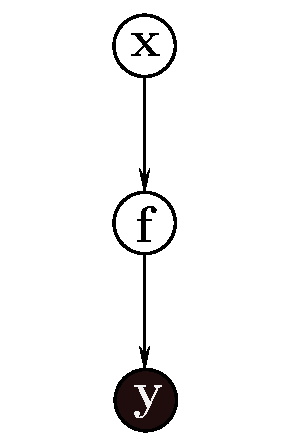
\includegraphics[width=25mm,height=33mm]{../../../vargplvm/tex/diagrams/Figure1}
%\end{l}
\end{figure}

\end{column}
\end{columns}

\vspace{0.3cm}

GP-LVM is trained by \textcolor{blue}{optimizing} 
      (\textcolor{blue}{not marginalizing} out) the latent variables

\begin{itemize}

\item Not proper density in the latent space 

\item Cannot select the latent dimensionality $Q$ 

\item It may overfit since it is not fully Bayesian 

\end{itemize}


}



\frame
{
\frametitle{Bayesian Gaussian process latent variables model}


\begin{columns}
\begin{column}[t]{8cm}

\begin{itemize}
\item Latent variable model: 

$$
\bfy  = \bff(\bfx)  + \bfepsilon 
$$

\item \textcolor{blue}{Bayesian training:} Integrate out both the latent mapping 
      and the latent space  

\begin{itemize}

\item Exact Bayesian inference is intractable 

\item But variational Bayesian inference is tractable 
 

\end{itemize}
\end{itemize}

\end{column}

\begin{column}[t]{4cm}
\begin{figure}
%\begin{l}
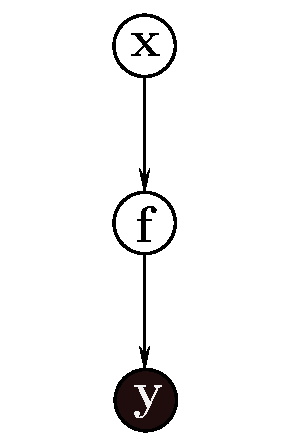
\includegraphics[width=25mm,height=33mm]{../../../vargplvm/tex/diagrams/Figure1}
%\end{l}
\end{figure}

\end{column}
\end{columns}

\vspace{0.5cm}
 

{\bf The variational method is applied as before. The only 
      difference is that now we have $D$ latent functions 
      (one for each observed output)
 and not just one}  

}




\frame
{
\frametitle{Bayesian Gaussian process latent variables model}


\textcolor{blue}{Automatic selection of the latent dimensionality}

\begin{itemize} 



\item Squared exponential ARD kernel

$$
k(\bfx,\bfx') = \sigma_f^2 \exp\left( - \frac{1}{2} \sum_{q=1}^Q
\alpha_q (x_q - x_q')^2 \right)
$$


\item Maximizing the variational lower bound w.r.t.\ 
      $\alpha_q$s allows to remove  
      redundant latent dimensions   

\end{itemize}

}


\frame
{
\frametitle{Experiments: Visualization}


\begin{itemize}


\item  Oil flow data: $1000$ training; $12$ dimensions; 3 known classes


\item Compare: 


 \begin{itemize} 

 \item Bayesian GP-LVM

\item Standard sparse GP-LVM 

\item Probabilistic PCA 
 
 \end{itemize}

 \end{itemize}

}


\frame
{
\frametitle{Experiments: Visualization}

Oil flow data 

%\begin{figure*}[ht]
\begin{center}
\begin{tabular}{cc}
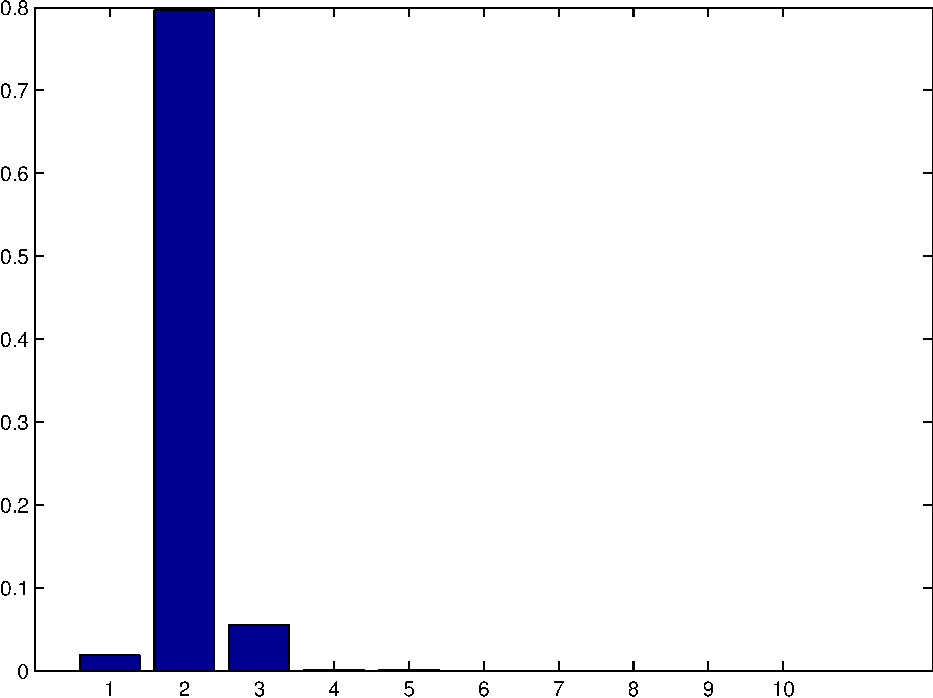
\includegraphics[width=42mm,height=35.5mm]
{../../../vargplvm/tex/diagrams/demOilVargplvmLengthScales1}&
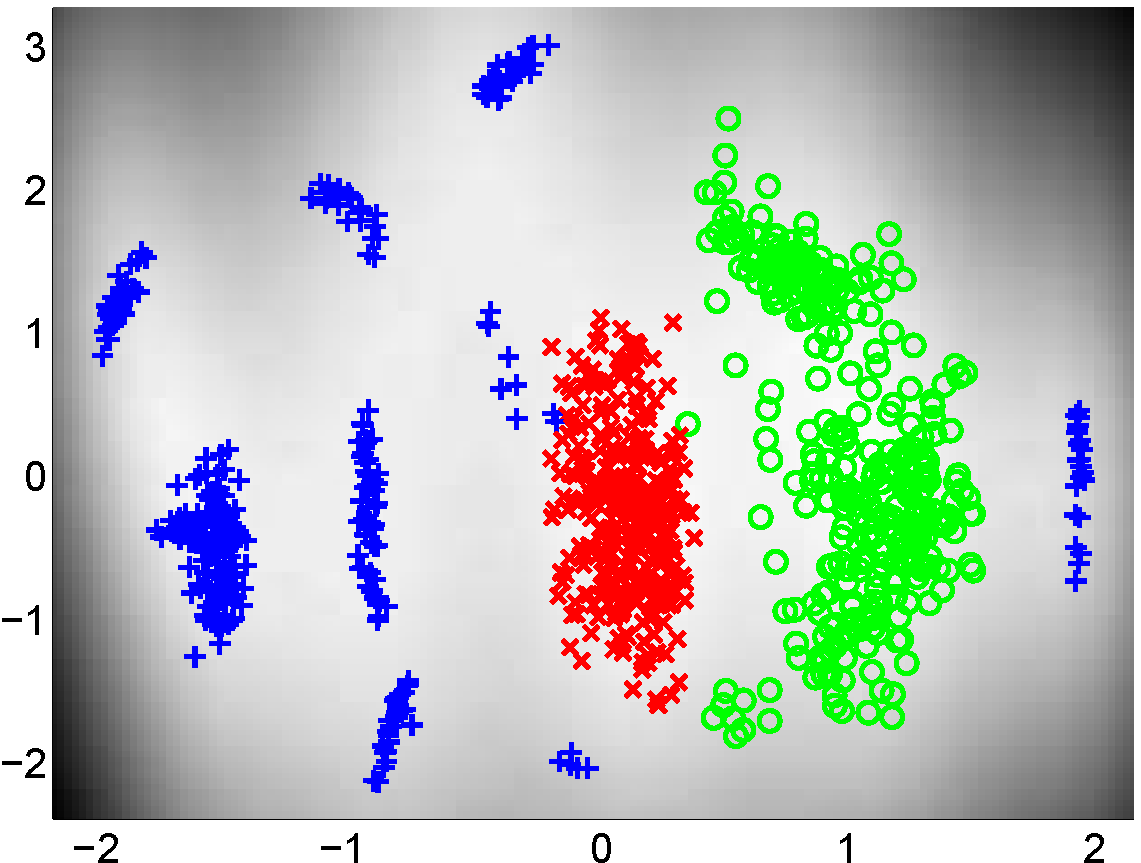
\includegraphics[width=42mm,height=35.5mm]
{../../../vargplvm/tex/diagrams/demOilVargplvm1}\\
($\alpha_q$s) & (Bayesian GP-LVM) 
\end{tabular}
%\caption{Panel (a) shows the inverse lengthscales found by applying the
%  Bayesian GP-LVM with ARD SE kernel on the oil flow data. Panel (b)
%  shows the visualization achieved by keeping the most dominant latent
%  dimensions (2 and 3) which have the largest inverse lengthscale
%  value. Dimension 2 is plotted on the
%  $y$-axis and 3 and on the $x$-axis. Plot (c) shows the visualization found
%  by standard sparse GP-LVM.
%\label{fig:Oil}}
\end{center}
%\end{figure*}

\begin{itemize}


\item Bayesian GP-LVM runs with $10$ latent dimensions

\item The \textcolor{red}{red}, \textcolor{green}{green} and 
     \textcolor{blue}{blue} points are the predicted
     means for the latent variables labeled with the known class 

\item \textcolor{red}{$7$ out $10$ latent dimensions are shrunk to zero} 

\item Visualization is shown for the dominant (with the largest
  inverse lengthscales) latent dimensions 

\end{itemize}   

}


\frame
{
\frametitle{Experiments: Visualization}

Oil flow data

%\begin{figure*}[ht]
\begin{center}
\begin{tabular}{ccc}
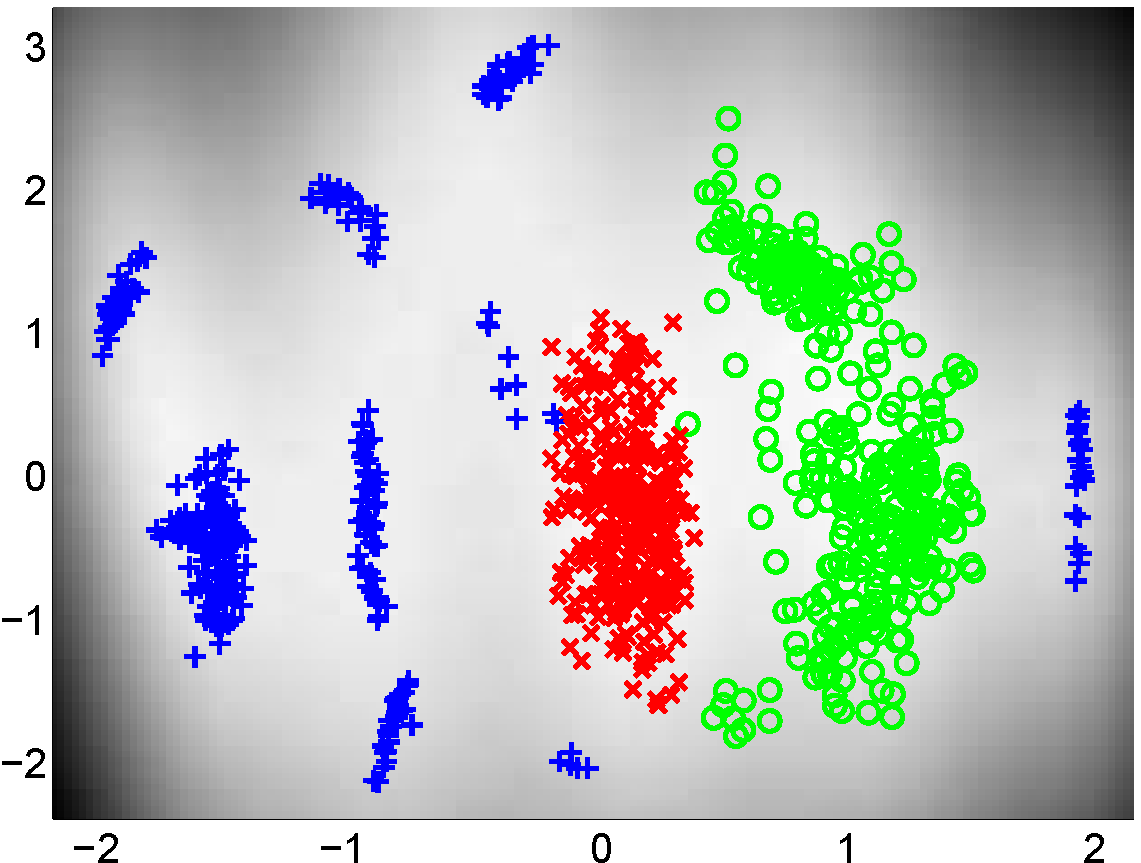
\includegraphics[width=34mm,height=30.5mm]
{../../../vargplvm/tex/diagrams/demOilVargplvm1} &
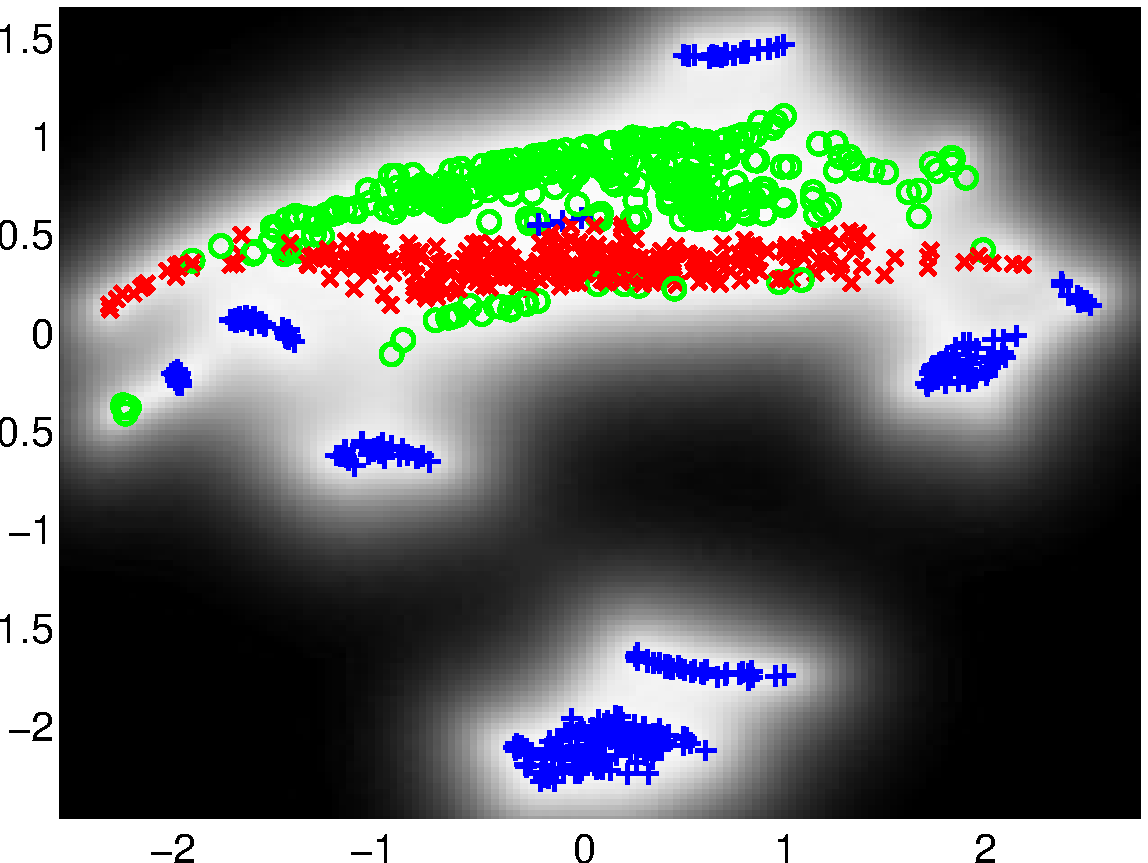
\includegraphics[width=34mm,height=30.5mm]
{../../../vargplvm/tex/diagrams/demOilFgplvm7} &
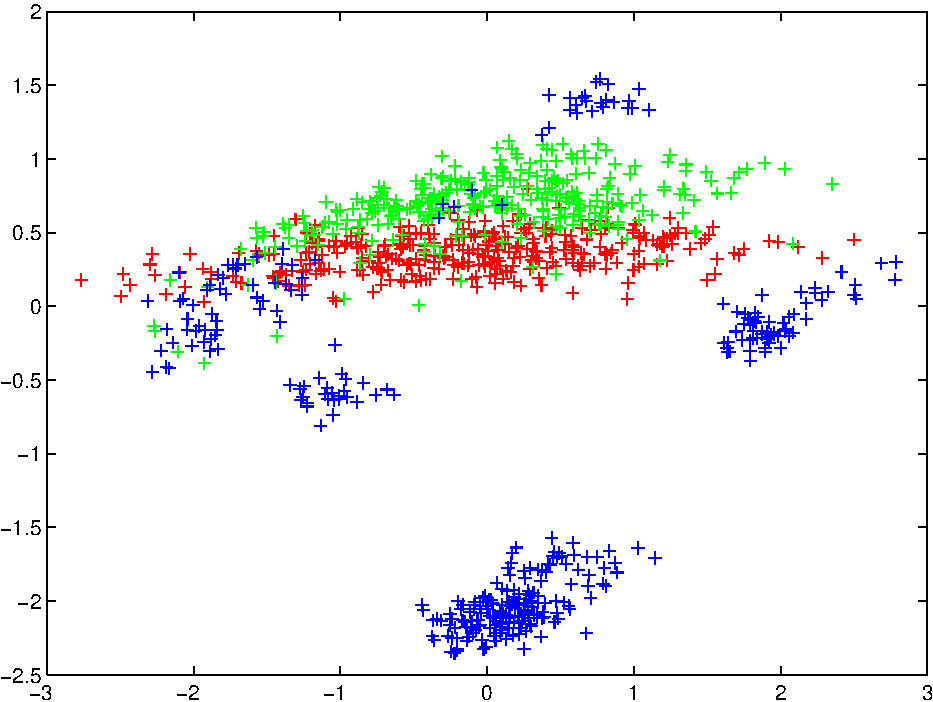
\includegraphics[width=34mm,height=30.5mm]
{../../../vargplvm/tex/diagrams/pcaOil}\\
(Bayesian GP-LVM) & (GP-LVM) & (PPCA)
\end{tabular}
%\caption{Panel (a) shows the inverse lengthscales found by applying the
%  Bayesian GP-LVM with ARD SE kernel on the oil flow data. Panel (b)
%  shows the visualization achieved by keeping the most dominant latent
%  dimensions (2 and 3) which have the largest inverse lengthscale
%  value. Dimension 2 is plotted on the
%  $y$-axis and 3 and on the $x$-axis. Plot (c) shows the visualization found
%  by standard sparse GP-LVM.
%\label{fig:Oil}}
\end{center}
%\end{figure*}


GP-LVM and Bayesian GP-LVM are both initialized based on PCA


}


%\frame
%{
%\frametitle{Experimetns with Bayesian GP-LVM}
%
%Inducing inputs $Z$ (pink diamonds)
%
%%\begin{figure}[ht]
%\begin{center}
%\begin{tabular}{c}
%\includegraphics[width=50mm,height=40mm]
%{../../../vargplvm/tex/diagrams/demOilVargplvm1WithInduc}\\
%(inverse lengthscales: $\alpha_q$s)
%%\caption{This plot shows the values of the inverse lengthscales
%%found by using the Bayesian GP-LVM with ARD SE kernel in Frey faces.  
%%\label{fig:BrendanInverseLenghScale}}
%\end{tabular}
%\end{center}
%%\end{figure}
%
%
%\begin{itemize}
%
%\item Inducing inputs are forced to be close to the means of the
%  variational distribution $q(X)$, i.e.\ close to the GP inputs
%
%\item This is consequence of the variarional method 
%      for standard sparse GPs (Titsias, 2009)
%
%\end{itemize}   
%
%}


\frame
{
\frametitle{Experiments: Predict missing values}

Frey faces: $1965$ images; $28 \times 20=560$ dimensions;
 $1000$ for training; $965$ for testing 


%\begin{figure*}[ht]
\begin{center}
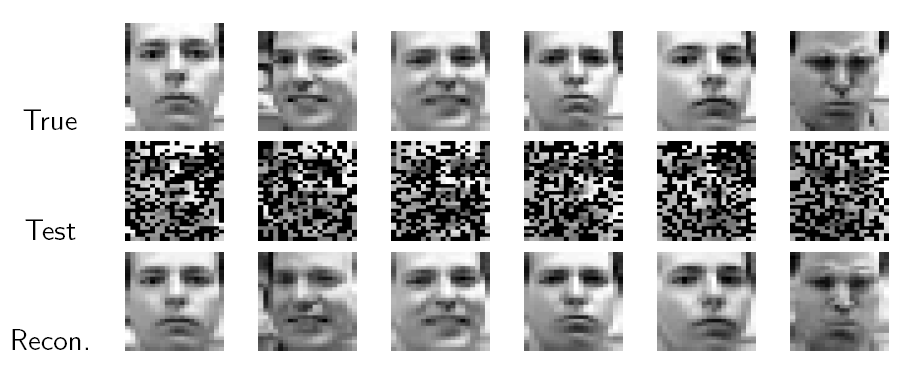
\includegraphics[width=1.1\textheight]
{../../../vargplvm/tex/diagrams/Frey2.PNG}
%\includegraphics[width=102mm,height=45.5mm]
%{../../../vargplvm/tex/diagrams/Frey2}
\end{center}
%\end{figure*}

\begin{itemize}

%\item Train with $1000$ images; reconstuct the missing pixels ($50\%$)
%  in the remaining $965$ test images 
%
%\item Row 1: original test images. Row 2: image with missing
%  pixels given to the algorithm. Row 3: reconstruct images


\item Bayesian GP-LVM is trained with $30$ latent dimensions, 
     \textcolor{blue}{mean absolute reconstruction error: $7.4003$}


\item Standard sparse GP-LVM is trained with several latent dimensions:
      $Q= 2, 5, 10, 30$. Errors: \textcolor{blue}{$10.5748, 9.7284, 19.6949, 19.6961$}


\end{itemize}   

}

\frame
{
\frametitle{Experiments: Generative classification}

\begin{itemize} 

\item  \textcolor{blue}{USPS digits dataset:} $16 \times 16$ images for all $10$ digits,  $7291$
training examples and $2007$ test examples

\item Run $10$ Bayesian GP-LVMs: one for each digit

\item Compute Bayesian class conditional densities in the test data of
  the form $p(\bfy_*|Y,\text{digit})$

\end{itemize}

Results: \textcolor{blue}{From $2007$ test images we have $95$ incorrectly
classified digits, i.e.\  4.73\% error}

}


%\frame
%{
%\frametitle{Experimetns with Bayesian GP-LVM}
%
%Fray faces: $1965$ images, $28 \times 20 =560$ dimensions
%
%%\begin{figure}[ht]
%\begin{center}
%\begin{tabular}{c}
%\includegraphics[width=50mm,height=40mm]
%{../../../vargplvm/tex/diagrams/demBrendanVargplvmLengthScales3}
%%\caption{This plot shows the values of the inverse lengthscales
%%found by using the Bayesian GP-LVM with ARD SE kernel in Frey faces.  
%%\label{fig:BrendanInverseLenghScale}}
%\end{tabular}
%\end{center}
%%\end{figure}
%
%
%
%\begin{itemize}
%
%\item Bayesian GP-LVM trained with 30 latent dimensions 
%     mean absolute reconstruction error: $7.4003$
%
%
%\item Standard GP-LVM trained with several latent dimensions:
%      $Q= 2, 5, 10, 30$. Errors: $10.5748, 9.7284, 19.6949, 19.6961$
%
%\end{itemize}   
%
%
%
%}



\frame
{
\frametitle{Summary/Future work}


Summary: 

\begin{itemize}

\item Variational framework to approximately integrate 
      out inputs in GPs 

\item Allows for Bayesian training of GP-LVM
        
\end{itemize} 

Future work: 

\begin{itemize}

\item Speed up optimization of the variational lower bound
%: Currently we use conjugate gradients
%           to jointly maximize the lower bound over variational 
%           and model parameters
%
%\begin{itemize} 
%
%\item Improvements: Find fixed point updates, 
%      explore the correlation structure of the optimized parameters
%
% \end{itemize}

 \item Learn non-parametric/non-linear 
         dynamical systems using GPs and variational Bayes    

\end{itemize}

}




\end{document}